\section{Χαρακτηριστικά εκδόσεων \en{OpenMP} 3.0 - 4.5}
\subparagraph{}
Η έκδοση του \emph{\en{OpenMP}} που ακολούθησε της 2.5, ήταν η 3.0. Η νέα έκδοση περιείχε σημαντικές προσθήκες και αλλαγές για τα δεδομένα του παράλληλου προγραμματισμού. Χαρακτηριστικά προηγούμενων εκδόσεων αναβαθμίστηκαν, ωστόσο τη σημαντικότερη αλλαγή αποτέλεσε η εισαγωγή της έννοειας των διεργασιών (\emph{\en{Tasking}}). Η επόμενη έκδοση του \emph{\en{OpenMP}} (4.0) κυκλοφόρησε τον Ιούλιο του 2013 και περιελάμβανε τα παρακάτω νέα χαρακτηριστικά:

\begin{itemize}
    \item \emph{\en{Threads affinity}},
    \item Ετερογενείς προγραμματισμός,
    \item Διαχείριση σφαλμάτων,
    \item Διανυσματικοποίηση μέσω \emph{\en{SIMD}},
    \item \emph{\en{User-Defined Recuctions (UDRs)}}
    \item Διεργασίας (\emph{\en{Tasking}}
\end{itemize}

Τα τελευταία χρόνια, η ανάγκη για εφαρμογές κατασκευασμένες με υψηλά επίπεδα παραλληλισμού είναι αυξημένη. Κύρια αιτία αποτελεί η ευκολία πρόσβασης σε μεγάλο όγκο δεδομένων από το ευρύ κοινό, οι μικρές εξαρτήσεις ανάμεσά στα δεδομένα, και η ανάγκη για εντατικούς υπολογισμούς στα δεδομένα αυτά. 
Λύση στο πρόβλημα αυξημένου φόρτου υπολογισμών αποτελεί η χρήση ετερογενών συστημάτων προγραμματισμού. 
Ωστόσο, παρά τα οφέλη της υλοποίησης και χρήσης τέτοιων συστημάτων σε ότι αφορά την απόδοση, ο προγραμματισμός εφαρμογών σε τέτοια συστήματα, δρα ανασταλτικά για την ευρεία χρήση τους. 
Το \emph{\en{OpenMP}} δημιούργησε τα κατάλληλα εργαλεία για την εξάλειψη προβλημάτων υλοποίησης. Με τη δημοσίευση της έκδοσης 4.0, προσέφερε την υποδομή για την υποστήριξη ετερογενών συστημάτων, καθώς η έκδοση περιλαμβάνει ένα σύνολο οδηγιών και φράσεων τα οποία χρησιμοποιούνται για τον προσδιορισμό ρουτίνων και δεδομένων, ικανών να μετακινηθούν σε μια συσκευή προορισμού (επιταχυντής), για να υπολογιστούν. Στόχος είναι η αύξηση των επιδόσεων υπολογισμού αλλά και η μείωση της κατανάλωσης ισχύος. 

Εκτός από την υποστήριξη ετερογενών συστημάτων, το \emph{\en{OpenMP}} την επεξεργασία δεδομένων μέσω διανυσματικοποίησης \emph{\en{SIMD}}. Η επεξεργασία \emph{\en{SIMD (Simple Instruction Multiple Data)}} εκμεταλλεύεται τον παραλληλισμό σε επίπεδο δεδομένων, πράγμα που σημαίνει ότι οι πράξεις που γίνονται σε ένα σύνολο στοιχείων διανύσματος, γίνονται ταυτόχρονα, μέσω απλών εντολών.

Στις ενότητες του κεφαλαίου που ακολουθούν, εκτός από την αναλυτικότερη περιγραφή των παραπάνω βασικών χαρακτηριστικών, γίνεται περιγραφή της έννοιας του \emph{\en{Thread Affinity}}, των \emph{\en{User-Defined Reductions}}, και των διεργασίών \emph{\en{(Tasking)}}.


\subsection{Διανυσματικοποίηση μέσω \emph{\en{SIMD}}}
\subparagraph{}

Κατά την διάρκεια εκτέλεσης ενός τυπικού προγράμματος από έναν μή παράλληλο υπολογιστή, οι εντολές που εκτελούνται είναι απλές, εφαρμοζόμενες σε απλά, μοναδιαία δεδομένα. Το μοντέλο αυτό ονομάζεται (\emph{\en{SISD - Single Instruction Single Data}}) και αποτελούσε για πολλά χρόνια το επικρατέστερο μοντέλο εκτέλεσης υλοποίησης και εκτέλεσης προγραμμάτων. Αποτελεί ένα απο τα τέσσερα μοντέλα της ταξινόμησης \emph{\en{Flynn}} που προτάθηκε το 1966\cite{flynn}. Τα άλλα τρία μοντέλα είναι: 
\begin{itemize}
\item{\emph{\en{SIMD - Single Instruction Multiple Data}}}
\item{\emph{\en{MISD - Multiple Instruction Single Data}}}
\item{\emph{\en{MIMD - Multiple Instructions Multiple Data}}}
\end{itemize}


Στο μοντέλο \emph{\en{Single Instruction Multiple Data (SIMD)}}, εκτελούνται απλές λειτουργίες για την τροποποίηση ενός συνόλου δεδομένων τοποθετημένων στη σειρά. Το σύνολο αυτών των δεδομένων ονομάζεται διάνυσμα.

Στο παρακάτω σχήμα παρουσιάζεται η πρόσθεση των στοιχείων δυο διανυσμάτων και η εκχώρηση των αποτελεσμάτων σε ένα τρίτο, με τον συμβατικό τρόπο, αλλά και με την χρήση \emph{\en{SIMD}} μεθόδου. Το πλεονέκτημα της δεύτερης μεθόδου είναι οτι οι \emph{\en{SIMD}} οδηγίες εκτελούνται το ίδιο γρήγορα με τις αντίστοιχες βαθμωτές. Με άλλα λόγια η πράξη του σχήματος, θα γίνει 4 φορές πιο γρήγορα στη δεύτερη περίπτωση.

\begin{figure}[h]
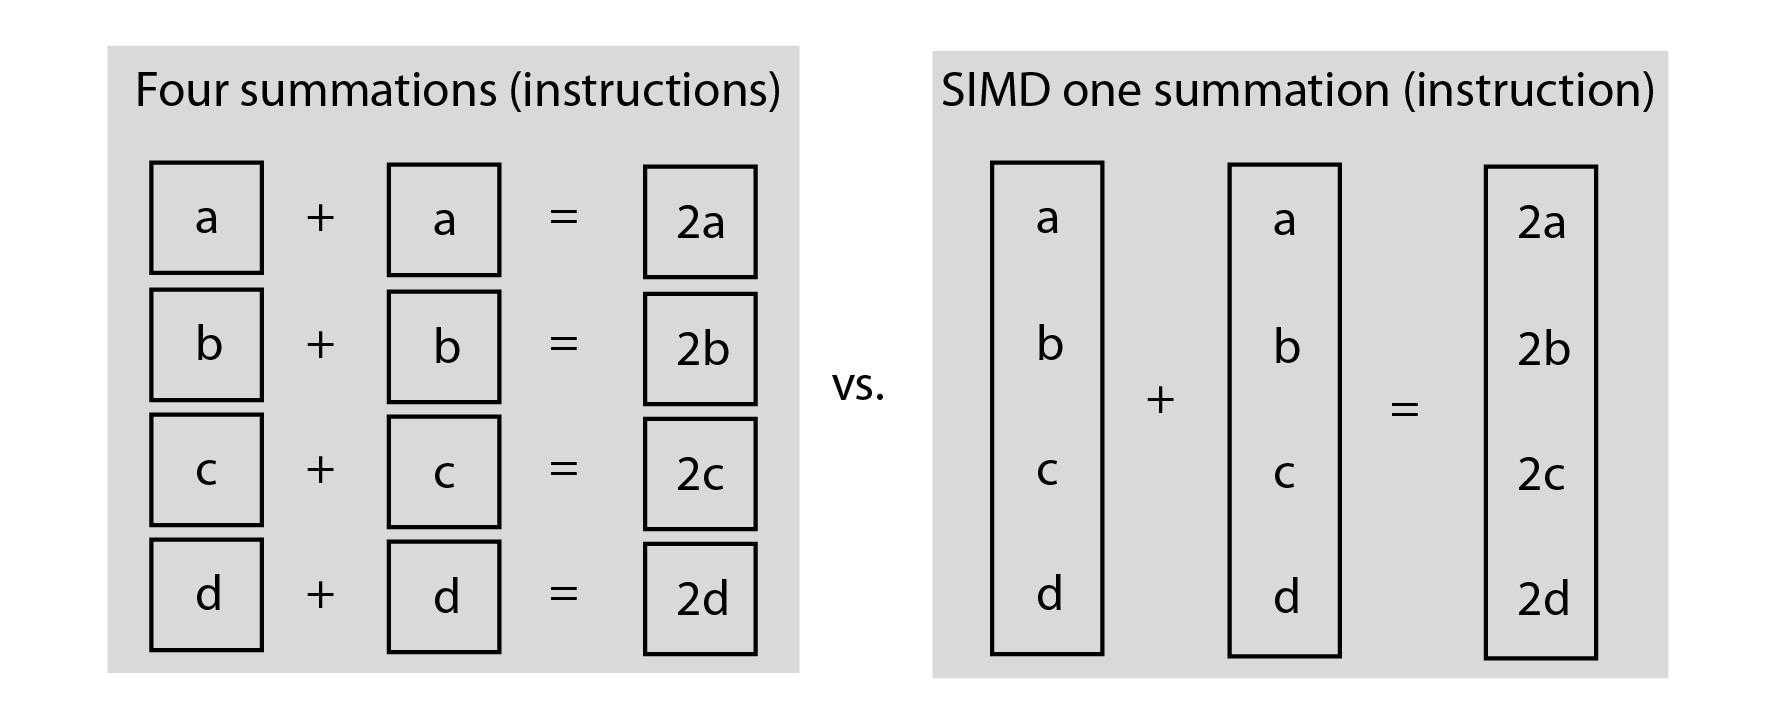
\includegraphics[width=\textwidth]{scalar_vs_simd}
\centering
\captionsetup{justification=centering, singlelinecheck=false}
	\caption{ Πρόσθεση διανυσμάτων βαθμωτά και με \en{SIMD}}
\label{fig:scalar_vs_simd}
\end{figure}

 Στο κεφάλαιο αυτό, περιγράφονται τα χαρακτηριστικά και οι δυνατότητες που είναι διαθέσιμες στο \emph{\en{OpenMP}} και αφορούν λειτουργίες διανυσματικοποίησης μέσω \emph{\en{SIMD}}. 

\clearpage
\subsubsection{Η οδηγία \emph{\en{simd}}}
\subparagraph{}
Αν ο μεταγλωττιστής δεν εφαρμόζει διανυσματικοποίηση ή δεν χρησιμοποιείται κάποια ειδική βιβλιοθήκη, τότε η επόμενη καλύτερη μέθοδος διανυσματικοποίησης είναι με τη χρήση του \emph{\en{OpenMP}}. Η διεπαφή εφοδιάζει το χρήστη με ένα σύνολο οδηγιών και φράσεων που σκοπό έχουν να ενημερώσουν το μεταγλωττιστή, να εκτελέσει παράλληλα ή με διανυσματικοποίηση, βρόγχους επανάληψης.

Βασικότερη οδηγία της διεπαφής αποτελεί η \textbf{\emph{\en{simd}}}. Εφαρμόζεται σε βρόγχους των οποίων η δομή είναι ίδια με την δομή των κοινών βρόγχων της \emph{\en{C++}}. Η εισαγωγή της οδηγίας \emph{\en{simd}} δίνει εντολή στο μεταγλωττιστή να δημιουργήσει έναν \emph{\en{simd}} βρόγχο.

Ιδιαίτερη προσοχή απαιτείται σε περιπτώσεις χρησης  μεταβλητών όπως δείκτες μέσα στο βρόγχο. Η λανθασμένη χρήσης τους μπορεί να προκαλέσει απροσδιόριστη συμπεριφορά.
Για παράδειγμα, στο παρακάτω τμήμα κώδικα, αν ο δείκτης \emph{\en{k}} ή \emph{\en{m}} είναι ταυτόσημος με τον δείκτη t, τότε αναμένονται λάθος αποτελέσματα.
\ \\
\selectlanguage{english}

\begin{lstlisting}[language=C++, caption={\el{Παράδειγμα κώδικα με} simd} , frame=tlrb]{Name}
void accumulate(int *t, int *k, int *m, int n) {
	#pragma omp simd
	for (int i = 0; i < n; ++i) {
		t[i] = k[i] + m[i];
	}
}
\end{lstlisting}
\selectlanguage{greek}


Στο παράδειγμα, η μεταβλητή \emph{\en{i}} είναι ιδιωτική. Η διαφορά με την ιδιωτική μεταβλητή ενός παράλληλου βρόγχου είναι οτι η ιδιωτικότητα αναφέρεται σε ένα \emph{\en{SIMD lane}}. Oι τιμές των διανυσμάτων \emph{\en{t, k, m}} είναι κοινόχρηστες. Το καταλληλότερο μήκος διανύσματος για την παραλληλοποίηση, εξαρτάται από την αρχιτεκτονική του μηχανήματος και επιλέγεται από αυτό.
\ \\
\subsubsection{Φράσεις οδηγίας \emph{\en{simd}}}
\subparagraph{}
Ένα σύνολο φράσεων ακολουθούμενων της οδηγίας \emph{\en{simd}} υποστηρίζεται απο το \emph{\en{OpenMP}}. Οι φράσεις \emph{\en{private, lastprivate, reduction, collapse, ordered}}, έχουν την ίδια χρησιμότητα που προαναφέρθηκε στην οδηγίες των προηγούμενων κεφαλαίων(πχ οδηγία διαμοιρασμού βρόγχου).
Το σύνολο των φράσεων που υποστηρίζονται από την οδηγία εμφανίζονται παρακάτω:
\selectlanguage{english}
\begin{lstlisting}[language=C++, caption={\el{Φράσεις που υποστηρίζονται από την οδηγία} \emph{simd}} , frame=tlrb]{Name}
private (list)
lastprivate (list)
reduction (reduction-identifier : list)
collapse (n)
simdlen (length)
safelen (length)
linear (list[: linear-step J)
aligned (list{:alignment])
\end{lstlisting}
\selectlanguage{greek}
\clearpage
\paragraph{Φράση \emph{\en{simdlen}}}
\subparagraph{}
Η φράση \emph{\en{simdlen}} δέχεται ως όρισμα ένα θετικό ακέραιο αριθμό που καθορίζει τον προτιμώμενο αριθμό επαναλήψεων ενός βρόγχου που θα εκτελούνται ταυτόχρονα. Επηρεάζει το μήκος του διανύσματος που χρησιμοποιείται από τις παραγόμενες \emph{\en{simd}} οδηγίες.

Η τιμή του ορίσματος είναι προτιμητέα αλλα όχι υποχρεωτική. Ο μεταγλωττιστής έχει την ελευθερία να αποκλίνει από αυτή την επιλογή και να επιλέξει διαφορετικό μήκος. Ελλείψη αυτής της φράσης ορίζεται μια προεπιλεγμένη τιμή που καθορίζεται από το μεταγλωττιστή. Σκοπός της φράσης \emph{\en{simdlen}} είναι να καθοδηγήσει τον μεταγλωττιστή. Χρησιμοποιείται από τον χρήστη όταν έχει καλή εικόνα των χαρακτηριστικών του βρόγχου και γνωρίζει όταν κάποιο συγκεκριμένο μήκος μπορεί να ωφελήσει στην απόδοση.

\paragraph{Φράση \emph{\en{safelen}}}
\subparagraph{}
Η φράση \emph{\en{safelen}} δέχεται ως όρισμα ένα θετικό ακέραιο αριθμό. Η τιμή αυτή καθορίζει το ανώτατο όριο του μήκους διανύσματος. Είναι το μήκος το οποίο είναι ασφαλές για τον βρόγχο. Το τελικό μήκος διανύσματος επιλέγεται από τον μεταγλωττιστή, αλλά δεν υπερβαίνει ποτέ την τιμή της φράσης \emph{\en{safelen}}.

Στο παρακάτω παράδειγμα απαιτείται η φράση \emph{\en{safelen}}. Πρόκειται για έναν βρόγχο που περιέχει δέσμευση στην προσπέλαση των στοιχείων του διανύσματος.
Πιο συγκεκριμένα, το διάβασμα του \emph{\en{[i-10]}} στην επανάληψη \emph{\en{i}} δεν μπορεί να υλοποιηθει, αν δεν ολοκληρωθεί η εγγραφή στο \emph{\en{k[i]}} της προηγούμενης επανάληψης.
 
\selectlanguage{english}

\begin{lstlisting}[language=C++, caption={\el{Παράδειγμα κώδικα με} simd} , frame=tlrb]{Name}
void dep_loop(float *k, float c, int n) {
	for (int i=10; i<n; i++) {
		k[i] = k[i-10] * c;
	}
}
\end{lstlisting}
\selectlanguage{greek}

\paragraph{H φράση \emph{\en{linear}}}
\subparagraph{}
Τα μοναδιαία δεδομένα εισάγονται σε διανύσματα. Στα διανύσματα εκτελούνται διεργασίες με τη χρήση οδηγιών \emph{\en{simd}} και εξάγονται τροποποιημένα δεδομένα. Οταν τα στοιχεία είναι προσβάσιμα με γραμμικό τρόπο, το διάνυσμα κατασκευάζεται εύκολα. Για παράδειγμα, δεδομένου ότι διατηρείται η ευθυγράμμιση των δεδομένων, μια απλή \emph{\en{simd}} οδηγία φόρτωσης και αποθήκευσης, χρησιμοποιείται για να γράψει και να διαβάσει διαδοχικά δεδομένα στο διάνυσμα.

Σε περιπτώσεις που τα δεδομένα παρατίθενται διαδοχικά στη μνήμη, η πρόσβαση στα στοιχεία γίνεται με \emph{μοναδιαίο βήμα}. Αν τα δεδομένα δεν είναι διατεταγμένα σε διαδοχικές θέσεις μνήμης, αλλά με τεχνητά κενά μεταξύ τους, τότε η προσέγγιση του μπορεί να γίνει με μεγαλύτερο βήμα. Στην περίπτωση αυτή το βήμα είναι ίσο με το κενό μεταξύ των στοιχείων.

\begin{figure}[h]
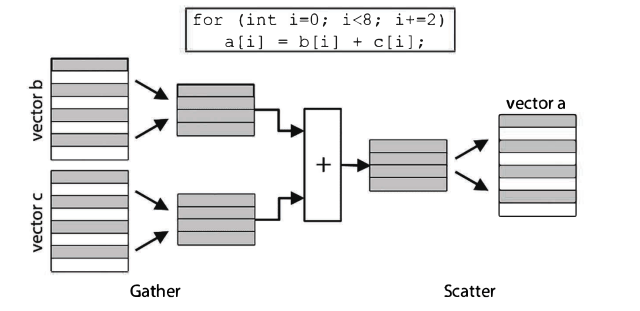
\includegraphics[width=0.9\textwidth]{linear_clause_simd}
\centering
\captionsetup{justification=centering, singlelinecheck=false}
	\caption{Σχηματική απεικόνιση φράσης \emph{\en{linear}}}
\label{fig:linear_clause_simd}
\end{figure}

Στην παραπάνω εικόνα περιγράφεται η λειτουργία συλλογής, επεξεργασίας και επανατοποθέτησης στη μνήμη, ενός συνόλου δεδομένων. Για την κατασκευή του διανύσματος, μια λειτουργία συγκέντρωσης διαβάζει γραμμικά αλλά με βήμα μεγαλύτερο του ενός. Ομοίως, μια δεύτερη λειτουργία γράφει τα δεδομένα του διανύσματος πίσω στη μνήμη γραμμικά, αλλα με βήμα μεγαλύτερο του ενος.


\paragraph{H φράση \emph{\en{aligned}}}
\subparagraph{}
Η ευθυγράμμιση των δεδομένων είναι σημαντική για την καλή απόδοση του προγράμματος. Εαν ένα στοιχείο διανύσματος δεν είναι ευθυγραμμισμένο σε διευθυνση μνήμης που είναι πολλαπλάσιο του μεγέθους του στοιχείου σε \emph{\en{byte}}, προκύπτει ένα επιπλέον κόστος καθυστέρησης για την τροποποίηση του στοιχείου αυτού.

Για παράδειγμα, σε ορισμένες αρχιτεκτονικές ενδέχεται να μην είναι δυνατή η φόρτωση και εγγραφή απο μια διεύθυνση μνήμης που δεν ειναι ευθυγραμμισμένη με το μέγεθος του δεδομένου που χρησιμοποιείται. Ετσι, οι λειτουργίες γίνονται κανονικά, αλλά με μεγαλύτερο κόστος. Σε περίπτωση διανυσματοκοποίησης μέσω της οδηγίας \emph{\en{simd}}, η επιλογή ευθυγράμμισης δεδομένων μπορεί να βελτιώσει την εκτέλεση.

Η φράση ευθυγράμμισης υποστηρίζεται τόσο από την οδηγία \emph{\en{simd}} όσο και από την οδηγία \emph{\en{declare simd}}. Η φράση δέχεται ως όρισμα μια λίστα μεταβλητών. ΗΗ τιμή της ευθυγράμμισης πρέπει να είναι ενας σταθερός ακέραιος αριθμός. Σε περίπτωση έλλειψης της φράσης, μια προεπιλεγμένη τιμή καθορίζεται από την υλοποίηση.

\clearpage
\subsubsection{Η σύνθετη οδηγία βρόγχου \emph{\en{SIMD}}}
\subparagraph{}
Η σύνθετη οδηγία βρόγχου \emph{\en{SIMD}}, συνδυάζει παραλληλισμό νημάτων και διανυσματικοποίηση μέσω\emph{\en{simd}}.

\selectlanguage{english}
\begin{lstlisting}[language=C++, caption={\el{Σύνθετη οδηγία βρόγχου με} \emph{simd}} , frame=tlrb]{Name}
#pragma omp for simd [clause[[,] clause] ...] new-line
	for-loops
\end{lstlisting}
\selectlanguage{greek}

\ \\
Οι επαναλήψεις ενός βρόγχου διαιρούνται σε τμήματα και διανέμονται στα νήματα μιας ομάδας νημάτων. Στη συνέχεια, τα τμήματα αυτά, εκτελούνται βάση την οδηγία \emph{\en{simd}} βρόγχου. Οι φράσεις που μπορούν να χρησιμοποιηθούν στην οδηγία διαμοιρασμού βρόγχου ή στην οδηγία \emph{\en{simd}} μπορούν να χρησιμοποιηθούν και σε αυτές τις σύνθετες οδηγίες.

Στη σύνθετη οδηγία, τμήματα επαναλήψεων του βρόγχου διανέμονται στην ομάδα νημάτων με τη μέθοδο που ορίζουν οι φράσεις διαμοιρασμού που χρησιμοποιούνται στην οδηγία διαμοιρασμού βρόγχου. Στη συνέχεια, τα τμήματα επαναλήψεων βρόγχου μετατρέπονται σε οδηγίες \emph{\en{simd}} με μέθοδο που ορίζεται από τις φράσεις για την οδηγία \emph{\en{simd}}. Τα παραπάνω φαίνονται σχηματικά στην επόμενη εικόνα:
\ \\
\begin{figure}[h]
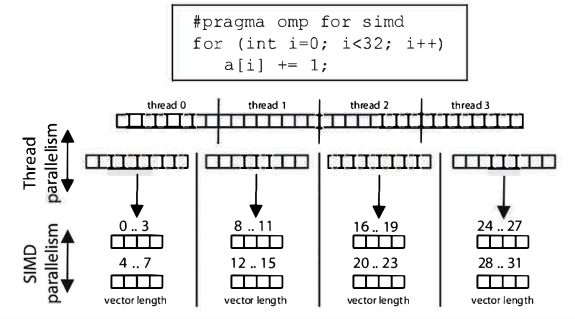
\includegraphics[width=0.9\textwidth]{for_simd}
\centering
\captionsetup{justification=centering, singlelinecheck=false}
	\caption{ Βήματα διεργασιών οδηγίας \emph{\en{for simd}}}
\label{fig:for_simd}
\end{figure}

Κάθε βρόγχος έχει ένα συγκεκριμένο ποσοστό εργασίας που πρέπει να εκτελέσει. Αν ο αριθμός των νημάτων αυξηθεί, το ποσοστό της εργασίας ανα νήμα θα μειωθεί. Προσθέτοντας παραλληλισμό \emph{\en{simd}}, δεν ειναι απαίτητη η βελτίωση της απόδοσης, ειδικά στις περιπτώσεις που ο \emph{\en{simd}} βρόγχος που ανήκει σε ένα νήμα, μειώσει το μήκος του.
\clearpage{}

\subsubsection{Συναρτήσεις \emph{\en{SIMD}}}
\subparagraph{}
Οι κλίσεις συναρτήσεων εντός της περιοχής βρόγχου \emph{\en{simd}} εμποδίζουν τη δημιουργία αποτελεσματικών \emph{\en{simd}} δομών. Στη χειρότερη περίπτωση η κλίση της συνάρτησης θα γίνει χρησιμοποιώντας βαθμωτά δεδομένα, και πιθανότατα θα επηρεάσει αρνητικά την αποτελεσματικότητα.

Για την πλήρη εκμετάλλευση του παραλληλισμού με διανυσματικοποίηση, για κάθε συνάρτηση που καλείται μέσα από ένα βρόγχο \emph{\en{simd}}, πρέπει ορίζεται μια ισοδύναμη έκδοσή της για εκτέλεση μέσα σε βρόγχους \emph{\en{simd}}. Ετσι, ο μεταγλωτιστής θα δημιουργήσει αυτή την ειδική έκδοση της συνάρτησης με \emph{\en{simd}} παραμέτρους και οδηγίες.

Η οδηγία \emph{\en{simd directive}} χρησιμοποιείται για να δημιουργήσει ο μεταγλωττιστής μια ή περισσότερες \emph{\en{simd}} εκδόσεις μιας συνάρτησης. Οι εκδόσεις αυτές χρησιμοποιούνται αποκλειστικά από βρόγχους \emph{\en{simd}}.


\paragraph{H οδηγία \emph{\en{declare simd}}}
\subparagraph{}
Η οδηγία \emph{\en{declare simd}} χρησιμοποιείται για να ενημερωθεί ο μεταγλωττιστής οτι μια συνάρτηση μπορεί να χρησιμοποιηθεί από μια περιοχή παραλληλισμού \emph{\en{simd}}.

\selectlanguage{english}
\begin{lstlisting}[language=C++, caption={\el{Οδηγία} \emph{declare simd}} , frame=tlrb]{Name}
#pragma omp declare simd [clause [[,] clause] ...] new-line
	function declaration definitions
\end{lstlisting}
\selectlanguage{greek}

\selectlanguage{english}
\begin{lstlisting}[language=C++, caption={\el{Φράσεις που υποστηρίζονται από} \emph{declare simd}} , frame=tlrb]{Name}
simdlen (length)
linear (list[: linear-step J)
aligned (list[:alignmentj)
uniform ( argument-list)
inbranch
notinbranch
\end{lstlisting}
\selectlanguage{greek}

Ο μεταγλωττιστής μπορεί να δημιουργήσει πολλές \emph{\en{simd}} εκδόσεις  μιας συνάρτησης και να επιλέξει την κατάλληλη για να κληθεί σε μια συγκεκριμένη τοποθεσία μιας κατασκευής \emph{\en{simd}}. Από τη μεριά του, ο χρήστης μπορεί να προσαρμόσει την λειτουργία μιας συνάρτησης με τη χρήση εξειδικευμένων φράσεων.

Υπάρχουν δύο περιορισμοί. Αν μια μεταβλητή αλλάζει ως αποτέλεσμα μιας τροποποίησης μιας φαινομενικά άσχετης μεταβλητής η συμπεριφορά είναι απροσδιόριστη. Επιπλέον, μια συνάρτηση που εμφανίζεται κάτω απο οδηγία \emph{\en{declare simd}}, δεν επιτρέπονται τα \emph{\en{exceptions}}.



\subsubsection{Χαρακτηριστικά παραμέτρων συνάρτησης \emph{\en{simd}}}
\subparagraph{}
Οι φράσεις \emph{\en{uniform, linear, simdlen, aligned}} χρησιμοποιούνται για τον καθορισμό χαρακτηριστικών στις παραμέτρους μιας συνάρτησης \emph{\en{simd}}. Εκτός από τη φράση \emph{\en{simdlen}}, οι μεταβλητές που εμφανίζονται στις υπόλοιπες φράσεις πρέπει να είναι παράμετροι της συνάρτησης για την οποία εφαρμόζεται η οδηγία.

Οταν μια παράμετρος εμπεριέχεται στη φράση \emph{\en{uniform}}, η τιμή της παραμέτρου είναι ίδια για όλες τις ταυτόχρονες κλίσεις κατά την εκτέλεση της οδηγίας \emph{\en{simd}} βρόχου. Η φράση \emph{\en{uniform(arg1, arg2)}} ενημερώνει τον \emph{\en{compiler}} να δημιουργήσει μια \emph{\en{simd}} συνάρτηση που προυποθέτει οτι αυτές οι δύο μεταβλητές είναι ανεξάρτητες από τον βρόγχο.
Η φράση \emph{\en{linear}} έχει διαφορετική σημασία όταν εμφανίζεται σε οδηγία \emph{\en{simd}}. Δείχνει οτι ένα όρισμα που μεταβιβάζεται σε μια συνάρτηση έχει γραμμική σχέση μεταξύ των παράλληλων επικλήσεων μιας συνάρτησης.
Κάθε \emph{\en{simd lane}} παρατηρεί την τιμή του ορίσματος στην πρώτη λωρίδα και προσθέτει την μετατόπιση της \emph{\en{simd}} λωρίδας από την πρώτη, επί το γραμμικό βήμα.
$$val_{curr} = val_1 + offset * step $$

Η φράση \emph{\en{inbranch}} χρησιμοποιείται όταν μια συνάρτηση καλείται πάντα μέσα σε ένα βρόγχο \emph{\en{simd}} και περιέχει \emph{\en{if condition}}. Ο μεταγλωττιστής πρέπει να αναδιαρθρώσει τον κώδικα για να χειριστεί την πιθανότητα ότι μια λωρίδα \emph{\en{simd}} μπορεί να μην εκτελέσει τον κώδικα μιας συνάρτησης.

Αντίθετα, η φράση \emph{\en{notinbranch}} χρησιμοποιείται όταν η συνάρτηση δεν εκτελείται ποτέ μέσα από ένα \emph{\en{if condition}} σε ένα \emph{\en{simd}} βρόγχο. Επιτρέπει τον μεταγλωττιστή κάνει μεγαλύτερες βελτιστοποιήσεις στην απόδοση του κώδικα μιας συνάρτησης που χρησιμοποιεί \emph{\en{simd}} οδηγίες.

\clearpage
\selectlanguage{english}
\begin{lstlisting}[language=C++, caption={\el{ Παράδειγμα χρήσης φράσεων} inbranch - notinbranch} , frame=tlrb]{Name}
#pragma omp declare simd inbranch
float pow(float x) {
	return (x * x);
}

#pragma omp declare simd notinbranch
extern float div(float);

void simd_loop(float *a, float *b, int n)
{
	#pragma omp simd
	for (int i=0; i<n; i++) {
		if (a[i] < 0.0 )
			b[i] = pow(a[i]);
		b[i] = div(b[i]);
	}
}
\end{lstlisting}
\selectlanguage{greek}